\documentclass[och, master]{SCWorks}

\usepackage[utf8]{inputenc}
\usepackage[T2A]{fontenc}
\usepackage[russian]{babel}

\usepackage{pdfpages}

\usepackage{hyperref}
\usepackage{amsfonts}
\usepackage{commath}
\usepackage{amsthm}
\usepackage{amssymb}
\usepackage{float}

\theoremstyle{plain}
\newtheorem{thethm}{Теорема}

\theoremstyle{plain}
\newtheorem{lemma}{Лемма}

\theoremstyle{plain}
\newtheorem{note}{Замечание}

\theoremstyle{definition}
\newtheorem{defn}{Определение} 

\newtheorem{exmp}{Пример}

\geometry{verbose,a4paper,tmargin=2cm,bmargin=2cm,lmargin=2.5cm,rmargin=1.5cm}

\hypersetup{
    colorlinks=true, %set true if you want colored links
    linktoc=all,     %set to all if you want both sect. and subsect. linked
    linkcolor=blue,  %choose some color if you want links to stand out
}

\author{Sharov Alex}

\newtheorem{problem}{Проблема}

\begin{document}

%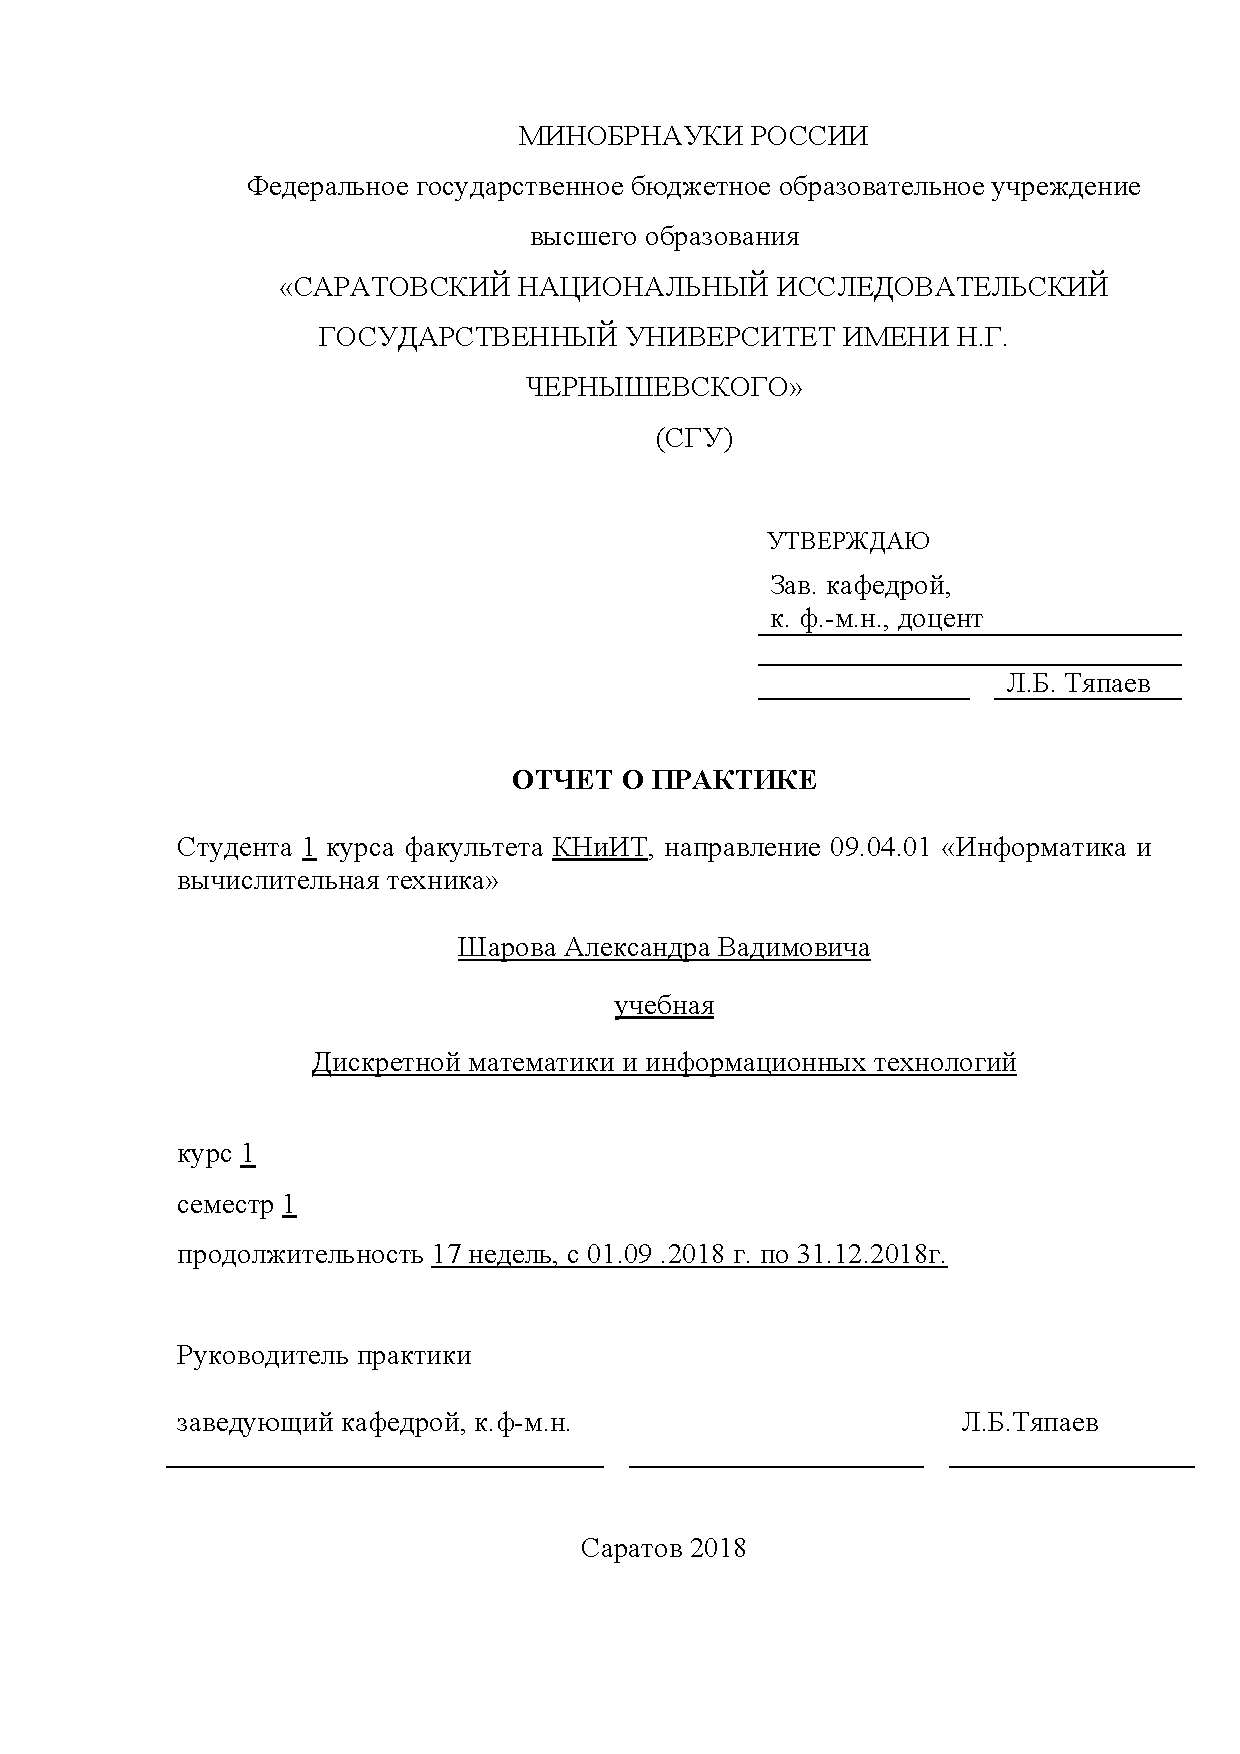
\includepdf[pages={1}]{titul.pdf}
\setcounter{tocdepth}{2}

\tableofcontents

	

\intro


Цель данной научно-исследовательской работы - попытка разобраться с гипотезой, которая была поставлена В. С. Анашиным и А. Ю. Хренниковым в книге Applied Algebraic Dynamics\cite{bib:dynamic:anashin} и подробно описана в первом разделе. Поскольку данная гипотеза - это открытая проблема, то нельзя заранее сказать о том, будет она доказана или опровергнута.

В течение семестра гипотеза была рассмотрена, а затем, чтобы в дальнейшем рассматривать гипотезу в терминах автоматов, была проведена работа по созданию алгоритма для преобразования детерминированных функций $f: \mathbb Z_p \rightarrow \mathbb Z_p$ в конечные автоматы. Задача о построение конечного автомата для детерминированной функции была поставлена и решена в курсовой работе для частной функции вида $f(x)=cx, c=\frac{n}{m}$, где $n,m \in \mathbb Z$.

Ближе к концу семестра была рассмотрена гипотеза Коллатца, которая, если ее переложить на язык $p$-адических функций, очень схожа с гипотезой рассмотренной в первом разделе.

Основной список используемой литературы для построения функции $f(x)=cx$ приведен в курсовой работе.

\section{Основная открытая проблема}

В книге \cite{bib:dynamic:anashin} В. С. Анашин и А. Ю. Хренников ставят следующую проблему, которую отмечают как открытую.


\begin{problem}\label{problem:general}
Существует ли полином $g$ над $\mathbb Z_2$ такой что композиция 

\begin{equation} \label{problem:1}
f(x)=g\bigg(\frac{x(x+1)}{2}\bigg)	
\end{equation}

\noindent транзитивна по $\pmod {2^{k}}$ для всех $k$.
\end{problem}

В начале семестра было рассмотрено предположение о том, что данную задачу можно рассматривать в терминах рядов Ван дер Пута и T-функций, но в последствии от этого было решено отказаться в пользу рассмотрения задачи в терминах автоматов. В терминах автоматов функцию $f(x)=\frac{x(x+1)}{2}$ можно рассматривать как некоторый ассинхронный автомат, а функцию $g$ как некоторый синхронный автомат.

\section{Гипотеза Коллатца (проблема $3x+1$)}
Помимо рассмотрения проблемы \ref{problem:general} в терминах автоматов был рассмотрен вариант переложения гипотезы Коллатца на термины $p$-адического анализа. После переложения гипотеза очень сильно стала напоминать исходную решаемую проблему. 

Перед постановкой гипотезы Коллатца в терминах $p$-адического анализа кратко объясним суть гипотезы. Для этого рассмотрим следующую последовательность чисел, называемую сиракузской последовательностью. Берём любое натуральное число $n \in \mathbb N$. Если оно чётное, то делим его на $2$, а если нечётное, то умножаем на $3$ и прибавляем $1$ (получаем $3n + 1$). Над полученным числом выполняем те же самые действия, и так далее. Гипотеза заключается в том, что какое бы начальное число $n$ мы ни взяли, рано или поздно мы получим единицу.

\begin{figure}[H]
\centerline{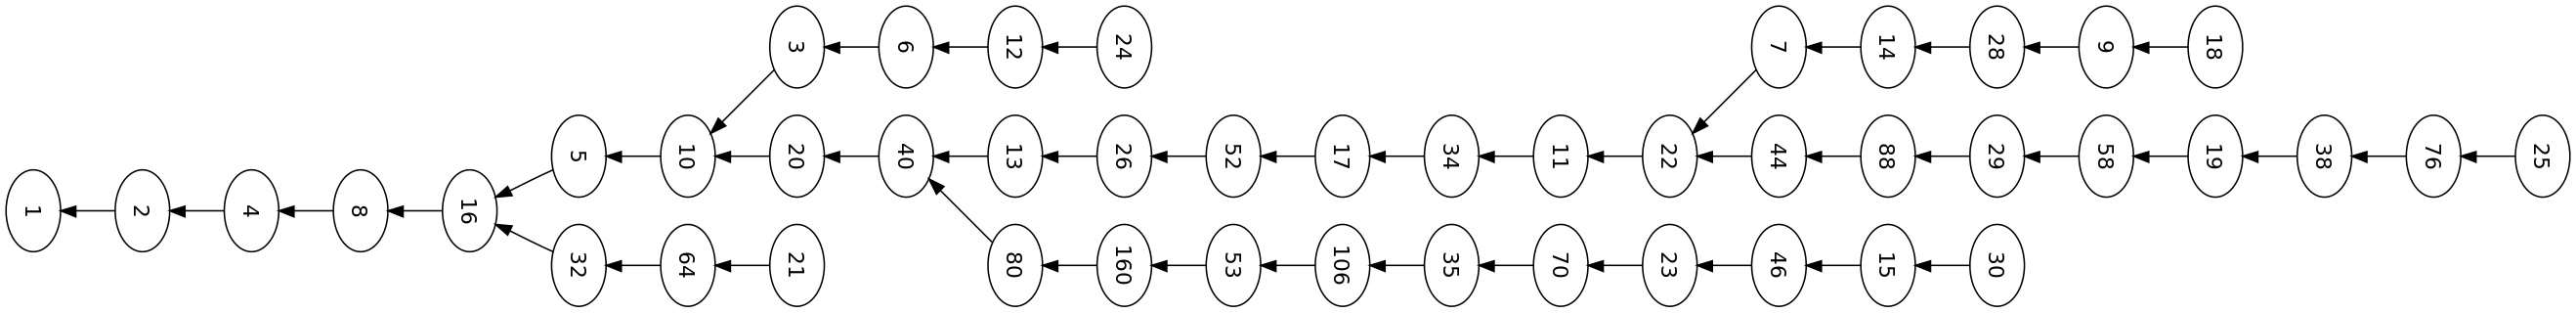
\includegraphics[width=1.0\linewidth]{img/seq}}
\caption{Пример сиракузской последовательности}
\label{img:1}
\end{figure}

\begin{figure}[H]
\centerline{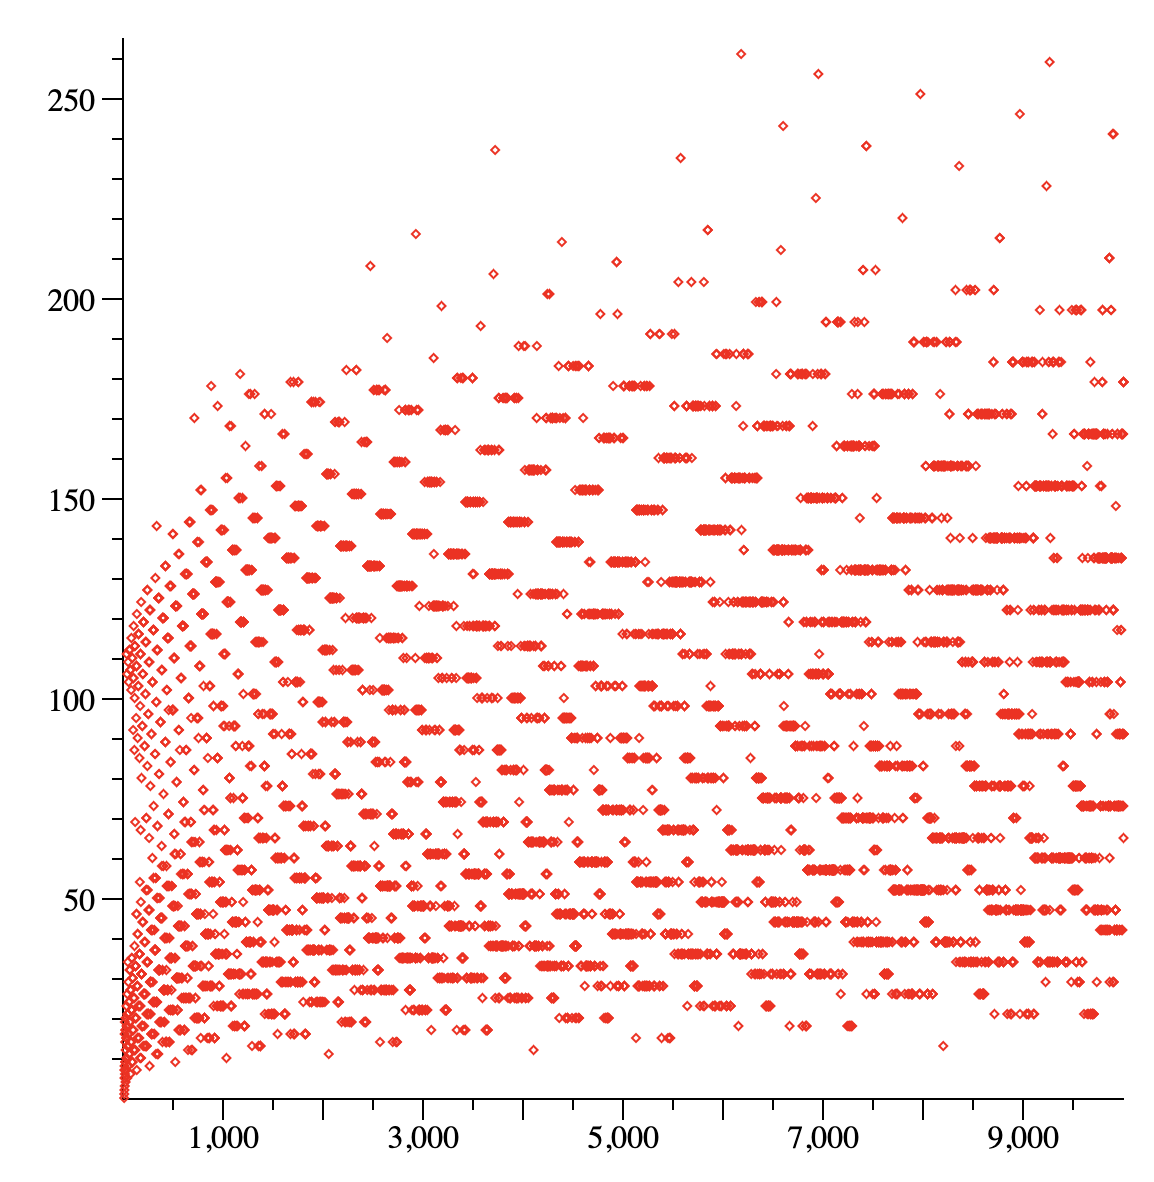
\includegraphics[width=0.5\linewidth]{img/len}}
\caption{Длины сиракузских последовательностей для чисел от 1 до 9999}
\label{img:2}
\end{figure}

Для постановки задачи в терминах $p$-адического анализа переформулируем гипотезу в виде следующей формулы:


\begin{equation} \label{problem:2}
\Phi_3(x)= \begin{cases}
   3x+1, x \equiv 1 \pmod 2
   \\
   \frac{x}{2}, x \equiv 0 \pmod 2
 \end{cases} \Leftrightarrow
\begin{cases}
   \frac{3x+1}{2}, x \equiv 1
   \\
   \frac{x}{2}, x \equiv 0
    \end{cases}
\end{equation}
 
\noindent Далее можно рассматривать вопрос о том, сохраняет ли функция $T_3$ меру Хаара и, если дополнительно ввести следующие функции:

$$ F: x \longmapsto \bigg[\frac{x}{2}\bigg], F: \mathbb N \rightarrow \mathbb N $$
$$ G: x=x_0+x_1p+x_2p^2+\ldots, x \longmapsto \frac{x-x_0}{p}$$

\noindent то можно рассматривать задачу об их биективности, совместимости и $1$-липшицевости.

В данных терминах гипотеза Коллатца очень напоминает гипотезу \ref{problem:general}.


\section{Построение автомата для функции вида $f(x)=cx$}

Для решения задачи \ref{problem:general} в терминах автоматов очень важно построить способ, который будет давать нам однозначное представление функции в виде автомата. Для этого были сделаны следующие шаги.


Для любого рационального числа $c=\frac{n}{m}$, где $n,m \in \mathbb Z$ и где $p$ не является делителем $m$, существует ограниченно-детерминированная функция $f: \mathbb Z_p \rightarrow \mathbb Z_p$ такая, что $f(x)=cx$. Обозначим через $\mathfrak{A}_c$ соотвествующий приведенный конечный автомат. Легко видеть, что для любой детерминированной функции $f: \mathbb Z_p \rightarrow \mathbb Z_p$ и слова $\alpha=a(1)a(2)\ldots a(l) \in E^l_p$ для соответствующей остаточной функции $f_\alpha (x)$ выполняется следующее соотношение:

\begin{equation} \label{automata:2}
f([\alpha]+p^lx)=[\beta]+p^l f_{\alpha}(x)
\end{equation}

\noindent где $\beta=b(1)b(2)\ldots b(l) =f(\alpha) \in E^l_p$:

\begin{equation} \label{automata:3}
\overbrace{\underbrace{a(1)\ldots a(l)}_{\alpha} \underbrace{x(1)x(2)\ldots}_{x}}^{[\alpha]+p^{l}x} \rightarrow
\boxed{f} \rightarrow \overbrace{\underbrace{b(1)\ldots b(l)}_{\beta} \underbrace{x(1)x(2)\ldots}_{x}}^{[\beta]+p^{l}f_{\alpha}(x)}
\end{equation}


\noindent Из соотношения \ref{automata:2} непосредственно следует формула для $f_{\alpha}(x)$:

\begin{equation} \label{automata:4}
f_{\alpha}(x)=\frac{f([\alpha]+p^{l}x)-[\beta]}{p^l}.
\end{equation}

\noindent Для начала опишем автомат $\mathfrak{A}_n$, где $n \in \mathbb N$. Применив формулу \ref{automata:4} к функции $f(x)=nx$, получим:

\begin{equation} \label{automata:5}
(nx)_{\alpha}=\frac{n([\alpha]+p^{l}x)-[\beta]}{p^l}	=nx+\frac{n[\alpha]-[\beta]}{p^l},
\end{equation}

\noindent где $[\beta]=n[\alpha] \pmod {p^l}$ (так как $f(\alpha)=\beta$). Следовательно, $n[\alpha]-[\beta]$ делится на $p^l$, и мы получаем более короткое представление:

\begin{equation} \label{automata:6}
(nx)_{\alpha}=nx+q,	
\end{equation}

\noindent где $q=\bigg[\frac{n[\alpha]}{p^l}\bigg] \in \{0, \ldots, n-1\}$, так как $n[\alpha]=p^l q+[\beta]$ и $[\alpha],[\beta] \in [0,p^l)$. Покажем, что $\forall q \in \{0, \ldots, n-1\} \quad \exists \alpha: \alpha \in E^l_p$, что  $q=\frac{n[\alpha]}{p^l}$.

\noindent Действительно, последнее эквивалентно следующему выражению:

\begin{equation} \label{automata:7}
p^l q \leq n[\alpha] \textless p^l q+ p^l.	
\end{equation}

\noindent Возьмем теперь достаточно больше $l$ так, чтобы выполнялось неравенство $p^l \textgreater n$, и положим $\alpha \in E^l_p$ равным $p$-ичной зависи числа $\bigg[\frac{p^l q}{n}\bigg]$, т.e. $[\alpha]=\bigg[\frac{p^l q}{n}\bigg]$. Тогда:

\begin{equation} \label{automata:8}
\frac{p^l q}{n} \leq [\alpha] \textless \frac{p^l q}{n} + 1 \Rightarrow p^l q \leq n[\alpha] \textless p^l q +n \Rightarrow p^l q \leq n[\alpha] \textless p^l q + p^l.
\end{equation}

\noindent Следовательно, слово $\alpha$ удовлетворяет условию (4) и $q=\bigg[\frac{n[\alpha]}{p^l}\bigg]$. Таким образом, показано что остаточные функции для $f(x)=nx$ полностью исчерпываются функциями $f^{(q)}(x)=nx+q$, где $q \in \{0, \ldots, n-1 \}$. Более того, все эти функции различны, поскольку $f^{(q)}(0) \neq f^{(q^{'})}(0)$ при $q \neq q^{'}$.

Такое наблюдение позволяет выбрать в качестве множества состояний приведенного автомата $\mathfrak{A}_n$, реализующего ограниченно-детерминированная функцию $nx$, множество $Q=\{0, \ldots, n-1 \}$. Опишем функцию переходов и функцию выходов автомата $\mathfrak{A}_n$. Применив формулу \ref{automata:4} к функции $f^{(q)}(x)=nx+q$ и однобуквенному слову $\alpha=a$, получим:


 \begin{equation} \label{automata:9}
 (nx+q)_{\alpha}=\frac{n(px+a)+q-b}{p}=nx+\frac{q+na-b}{p}	
 \end{equation}
 
\noindent где $b=na+q \pmod p$. Тогда $(nx+q)_\alpha = nx + q^{'}$, где $q^{'}=\frac{q+na-b}{p}$, и в автомате $\mathfrak{A}_n$ переход $q \xrightarrow{a/b} q^{'}$ существует тогда и только тогда, когда выполнено равенство:
 
 \begin{equation} \label{automata:10}
 	q+na=pq^{'}+b
 \end{equation}

\noindent Так как $q^{'} \in [0, n)$ и $b \in [0,p)$, то из равенства \ref{automata:10} следует, что

\begin{equation}
q^{'}=p^{-1}(q-a) \pmod n, \\
b=n^{-1}(a-q) \pmod p	
\end{equation}

\noindent где $p^{-1}$ - это обратный элемент для $p$ в кольце целых чисел по модулю $n$, а $n^{-1}$ - это обратный элемент для элемента $n$ в кольце целых чисел по модулю $p$. Оба элемента существуют, поскольку $n$ и $p$ - взаимно простые числа.


\conclusion
В дальнейшей научной работе планируется формализовать способ получения автомата для любого полинома и последующее применение полученных результатов к проблеме \ref{problem:general}.


\bibliographystyle{biblio/ugost}
\bibliography{biblio/biblio}

\end{document}